\chapter{先行研究}
\label{chap:prior}
本論文の議論のベースとなる,岡田らの従来手法と島田らが提案したトポロジカルマップの形式,単語の組み合わせによる経路の表現であるシナリオについて述べたのち,春山らの視覚に基づいて目的地まで自律移動するシステムについて述べる.
\section{視覚と行動の end-to-end 学習により経路追従行動をオンラ
インで模倣する手法}
岡田らの手法では,メトリックマップに基づく経路追従行動を視覚を入力とした行動へ模倣するために,end-to-end学習を用いた手法を提案している.
ロボットは経路を自律移動するのと同時に学習を行う.
手法に基づいて構築されたシステムを\figref{fig:okada_sys}に示す.

\begin{figure}[htbp]
  \centering
   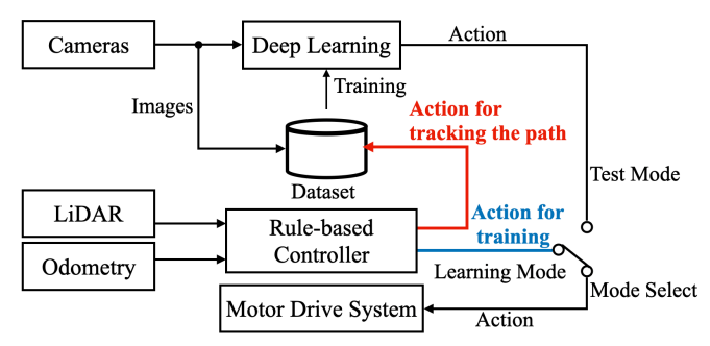
\includegraphics[width=100mm]{images/pdf/okada/method_sys.pdf}
   \caption[Structure of the Okada and others proposed system]{Structure of the Okada and others proposed system(Quoted from\cite{okada2020})}
   \label{fig:okada_sys}
\end{figure}

訓練時には,ROS の navigation パッケージ \cite{ros}を使用して,設定した経路を追従する.
ロボットの並進速度は 0.2 m/sに固定する.
その際,ロボットに取り付けたカメラから取得した RGB 画像とルールベース制御器が出力するヨー方向の角速度をペアにして, 0.2 秒の周期でデータセットに追加する.
収集には 3 台のカメラを使用することで,データの多様性を高めるとともに過学習を防ぐ効果を狙っている.
また,左右のカメラ画像に対するヨー方向の角速度には経路復帰を補助するためのオフセット(\(\pm 0.2\)rad/s)を加える.

\newpage
\figref{fig:okada_net}に岡田らの従来手法における学習器のネットワーク構造を示す.
% 学習器は入力をRGB画像データ,出力をロボットのヨー方向の角速度としている.
ネットワークは,入力層 1,畳み込み層 3,全結合層 2,出力層 1 の全7層で構成される.
データセットからはバッチサイズ 8 で教師データを抽出し, end-to-end 学習を行う.

\begin{figure}[htbp]
    \centering
     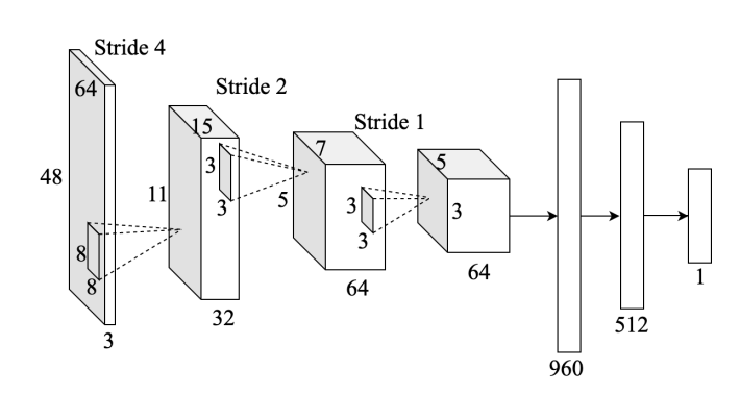
\includegraphics[width=100mm]{images/pdf/okada/network.pdf}
     \caption[Structure of the network Okada and others used]{Structure of the network Okada and others used (Quoted from \cite{okada2020})}
     \label{fig:okada_net}
\end{figure}

学習器の訓練後は,中央のカメラから得た RGB 画像を入力とし,出力されるヨー方向の角速度を用いて経路を追従する.
% この手法は実ロボットを用いて有効性が調査されており,\figref{fig:cource}に示す学習した経路を,画像のみを入力とした学習器の出力で自律移動できることが確認されている.
この手法は実ロボットを用いて有効性が調査されており,学習した経路を画像のみを入力とした学習器の出力で自律移動できることが確認されている.
% \begin{figure}[htbp]
%   \centering
%    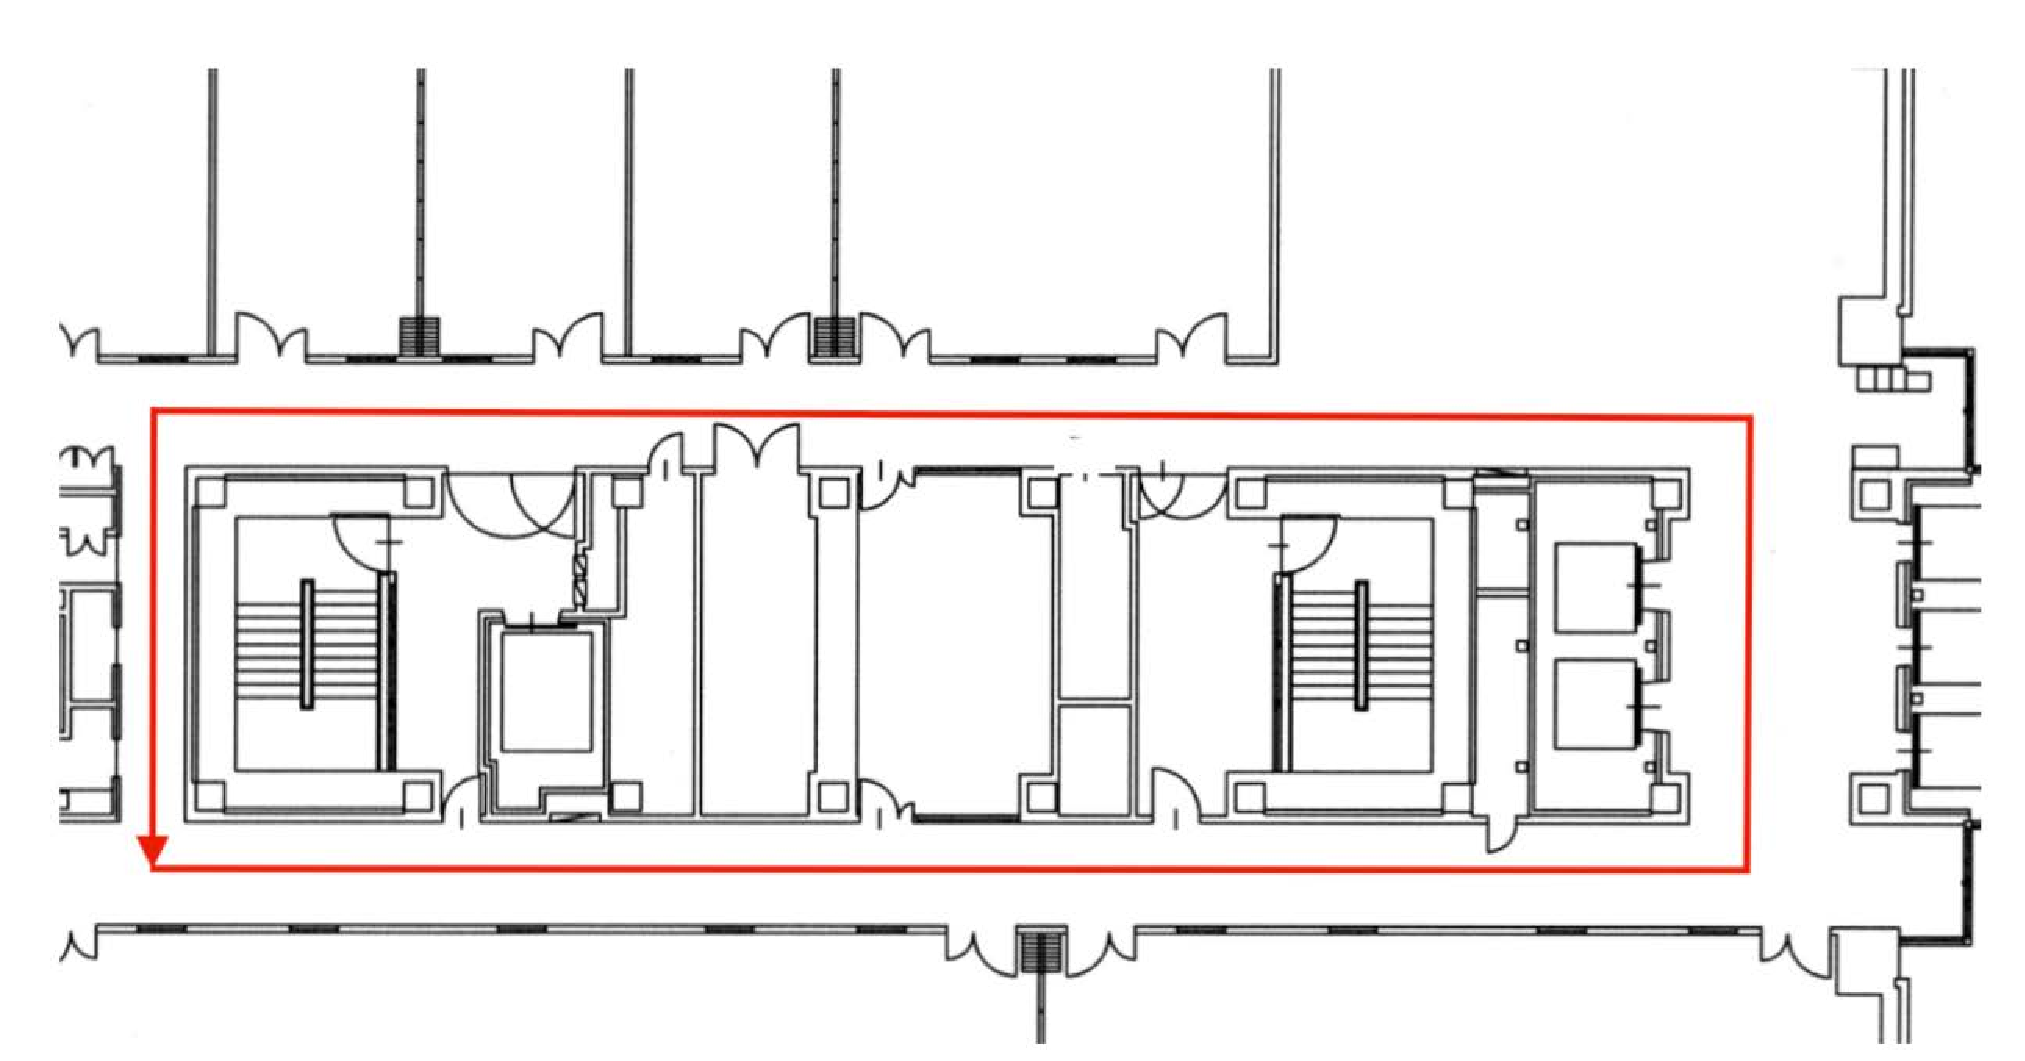
\includegraphics[width=80mm]{images/pdf/okada/cource.pdf}
%    \caption{Target path used in the experiment(Quoted from \cite{okada2020})}
%    \label{fig:cource}
% \end{figure}

\section{トポロジカルマップとシナリオ}
\subsubsection{トポロジカルマップ}
トポロジカルマップとは,環境をランドマークや特徴的な箇所をノードとし,その繋がりをエッジで表現した地図である.
島田らが提案したトポロジカルマップでは,ノードは通路の特徴的な箇所に配置され,エッジはノード間を接続する.
ノードにはID,通路の特徴(Type),エッジIDと相対角度(Edge)のデータが含まれ,エッジにはIDのみが含まれる.
この形式は道案内に関するアンケート結果に基づいており,人が道案内で「通路の特徴」や「向いている方向」を重視することが明らかになったことから設計された.

\begin{figure}[htbp]
  \centering
   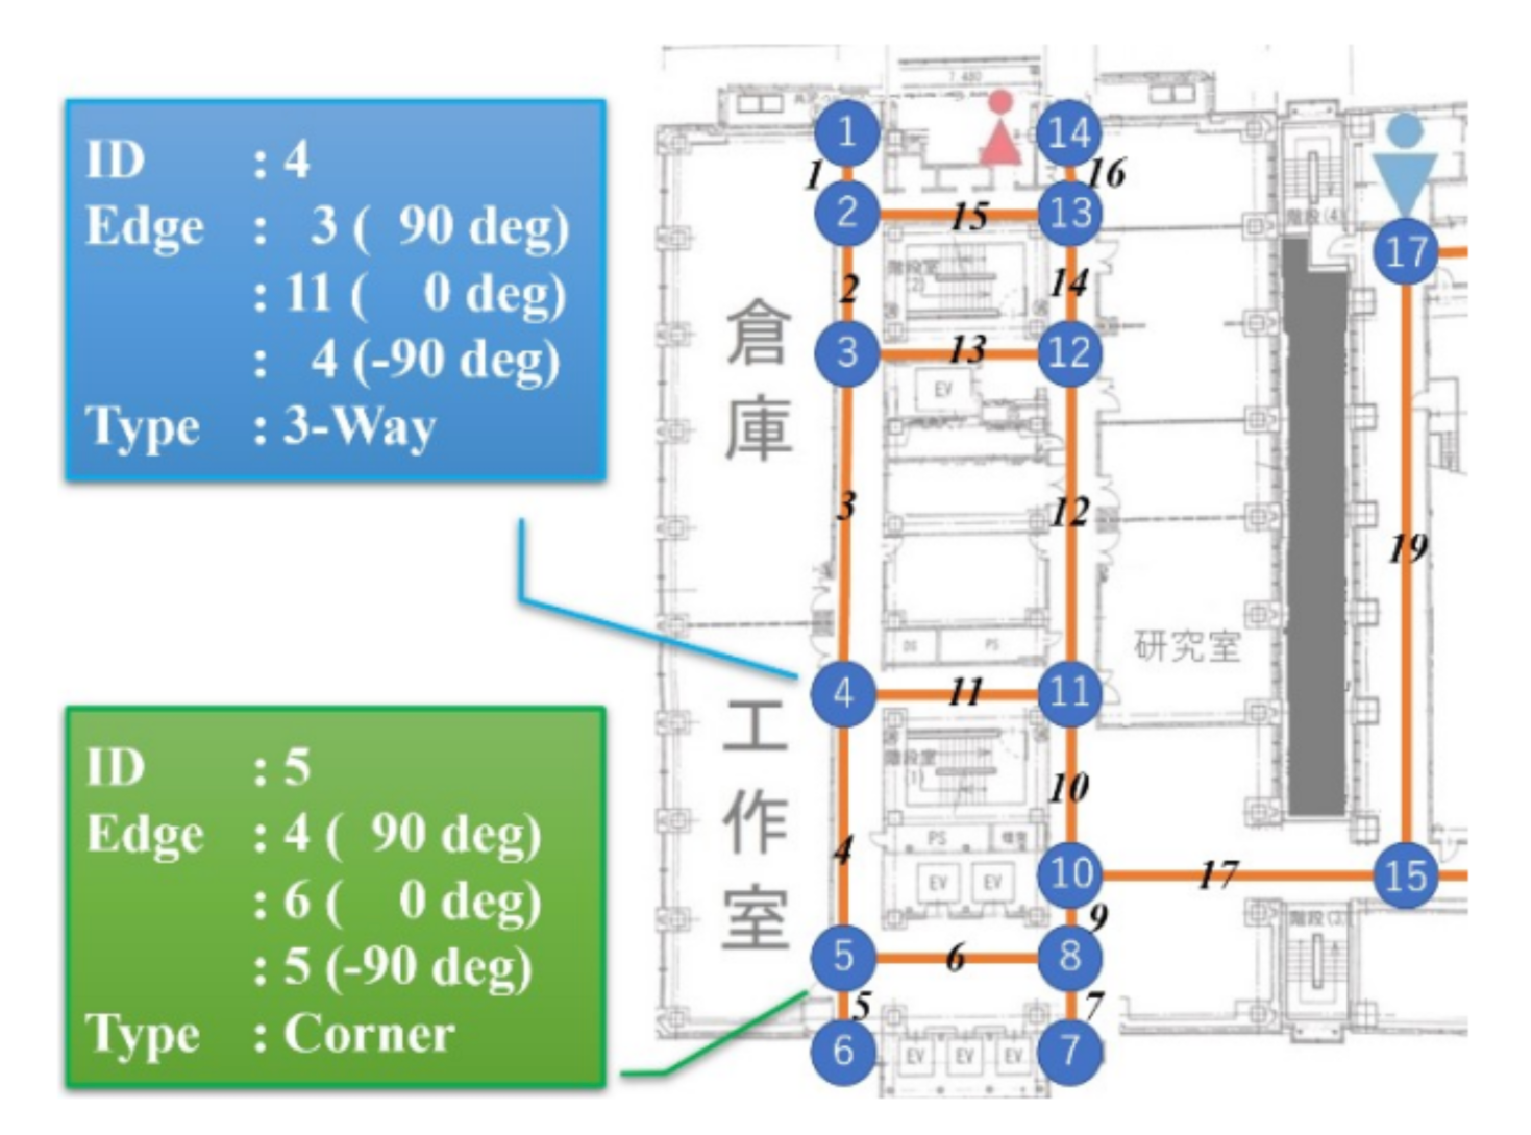
\includegraphics[width=80mm]{images/pdf/shimada/topo.pdf}
   \caption[Topological map format proposed by Shimada and others]{Topological map format proposed by Shimada and others(Quoted from\cite{shimada2020})}
   \label{fig:topo}
\end{figure}

\clearpage
\subsubsection{シナリオ}
シナリオは,トポロジカルマップ上の目的地までの経路を「条件」と「行動」の組み合わせで表現する手法である.
「条件」は「次の角」や「突き当たりまで」などを指し,「行動」は「直進」や「右折」などを指す.
この形式はトポロジカルマップ同様に道案内に関するアンケート結果に基づいており,人が「条件」と「行動」を組み合わせて道案内をすることが明らかになったことから設計された.
例として,特定の経路はと表現される.

\begin{figure}[htbp]
  \centering
   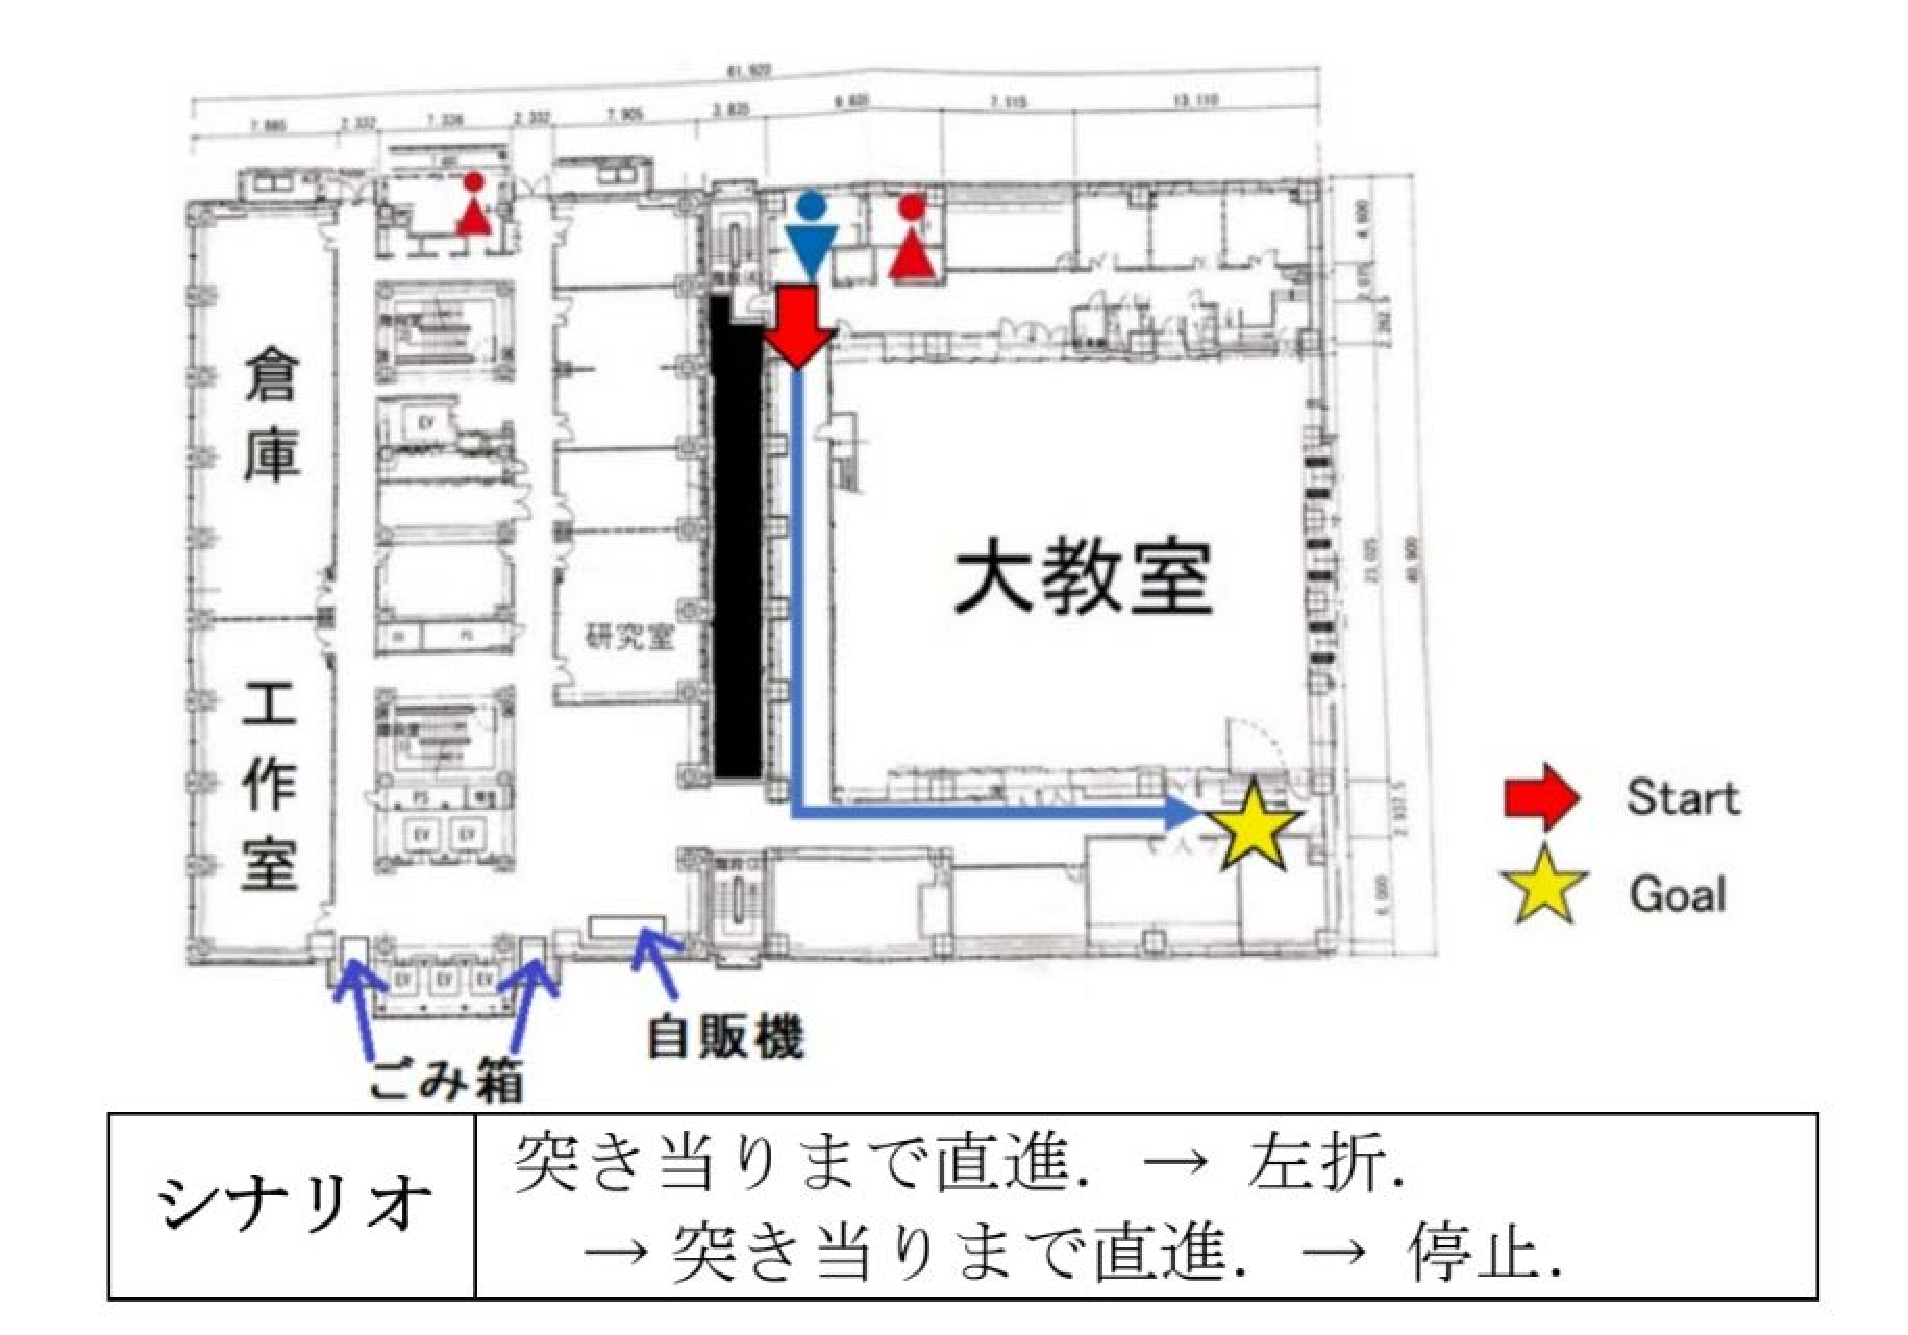
\includegraphics[width=90mm]{images/pdf/shimada/scenario.pdf}
   \caption{Topological map format proposed by Shimada and others(Quoted from\cite{shimada2020})}
   \label{fig:topo}
\end{figure}
\section{視覚に基づいて目的地まで自律移動するシステム}
春山らは,カメラ画像とトポロジカルマップから作成されるシナリオに基づいて,目的地まで自律移動するシステムを構築している.
提案されたシステムは,

1)カメラ画像と目標方向を与えることで,経路を追従するモジュール(以後,経路追従モジュールと呼ぶ)

2)シナリオを分解し,「条件」と「行動」を抽出するモジュール(以後,シナリオモジュールと呼ぶ)

3)カメラ画像から通路の特徴を分類するモジュール(以後,通路分類モジュールと呼ぶ)

の3つのモジュールで構成されており,それぞれについて述べる.
\subsection{経路追従モジュール}
このモジュールは,岡田らの手法から目標方向のデータを加えることで,分岐路で経路を選択し,移動する機能を追加したものである.
ここで目標方向とは,目標とする進行方向(「直進」や「右折」)を表す.
学習時は,カメラ画像とルールベース制御器が出力するヨー方向の角速度,目標方向を 0.2 秒周期でデータセットに加える.
データセットから抽出するバッチサイズや,カメラ画像の解像度は岡田ら手法と同様である.
データセットの収集には藤原らが提案した,データセットに加えるデータの不均衡を改善する手法,学習時に積極的な蛇行する手法を採用する.
\subsection{シナリオモジュール}
\subsection{通路分類モジュール}
このモジュールでは,ニューラルネットワークを用いることで,カメラ画像を入力として,通路の特徴を分類する.
データセットの収集をするために,ロボットをルールベース制御器に基づいて走行させる.
その際に,フレーム数 16 ,画像サイズ 64 × 48の連続したカメラ画像と通路の分類ラベルを1組として,0.125 秒周期でデータセットに加える.
通路の分類ラベルのアノテーションはルールベース制御器から出力されるラベルによって自動的に行う.
データセット内の不均衡を改善するために,クラス間のデータ数によって重み付けを行うコストアプローチを導入している.

実ロボットを用いた実験により,ロボットを目的地まで到達可能か検証されている.
実験では島田ら用いた 50 例のシナリオの中から,7例が用いられており,そのすべてでロボットが目的地へ到達できることが確認されている.